\chapter{Application overview}
\label{ch:applicationoverview}
\markboth{Application overview}{}

\begin{flushright}
	{\smaller
		\textit{C'è qualcuno che può rompere il muro del suono,\\ mentre tutto il mondo si commenta da solo.}\\
		-- L. Ligabue}
\end{flushright}

In this Chapter an overview of the \gls{acr:Adopt} software, and its reference library \gls{acr:Jpad} is presented.\\
\gls{acr:Adopt} is a Java-based desktop application developed at the University of Naples Federico II, conceived as a fast, reliable and user friendly computational aid for aircraft designers in the conceptual and preliminary design phases. The ultimate goal of such a tool is to perform a parametric, multi-disciplinary analysis of an aircraft and then search for an optimized configuration. The search domain boundaries are usually defined by the user through a set of specifyed parameters. An important design requirement of  \gls{acr:Adopt} is related to its interoperability with other engineering analysis tools. In fact, the application can be easily integrated into a comprehensive aircraft optimization cycle. This is made possible because  \gls{acr:Adopt} can be launched both in \gls{acr:gui} and command line mode. Much care has been given to input/output and configuration files to increase the possible uses of the software.

\begin{figure}[H]
	\centering
	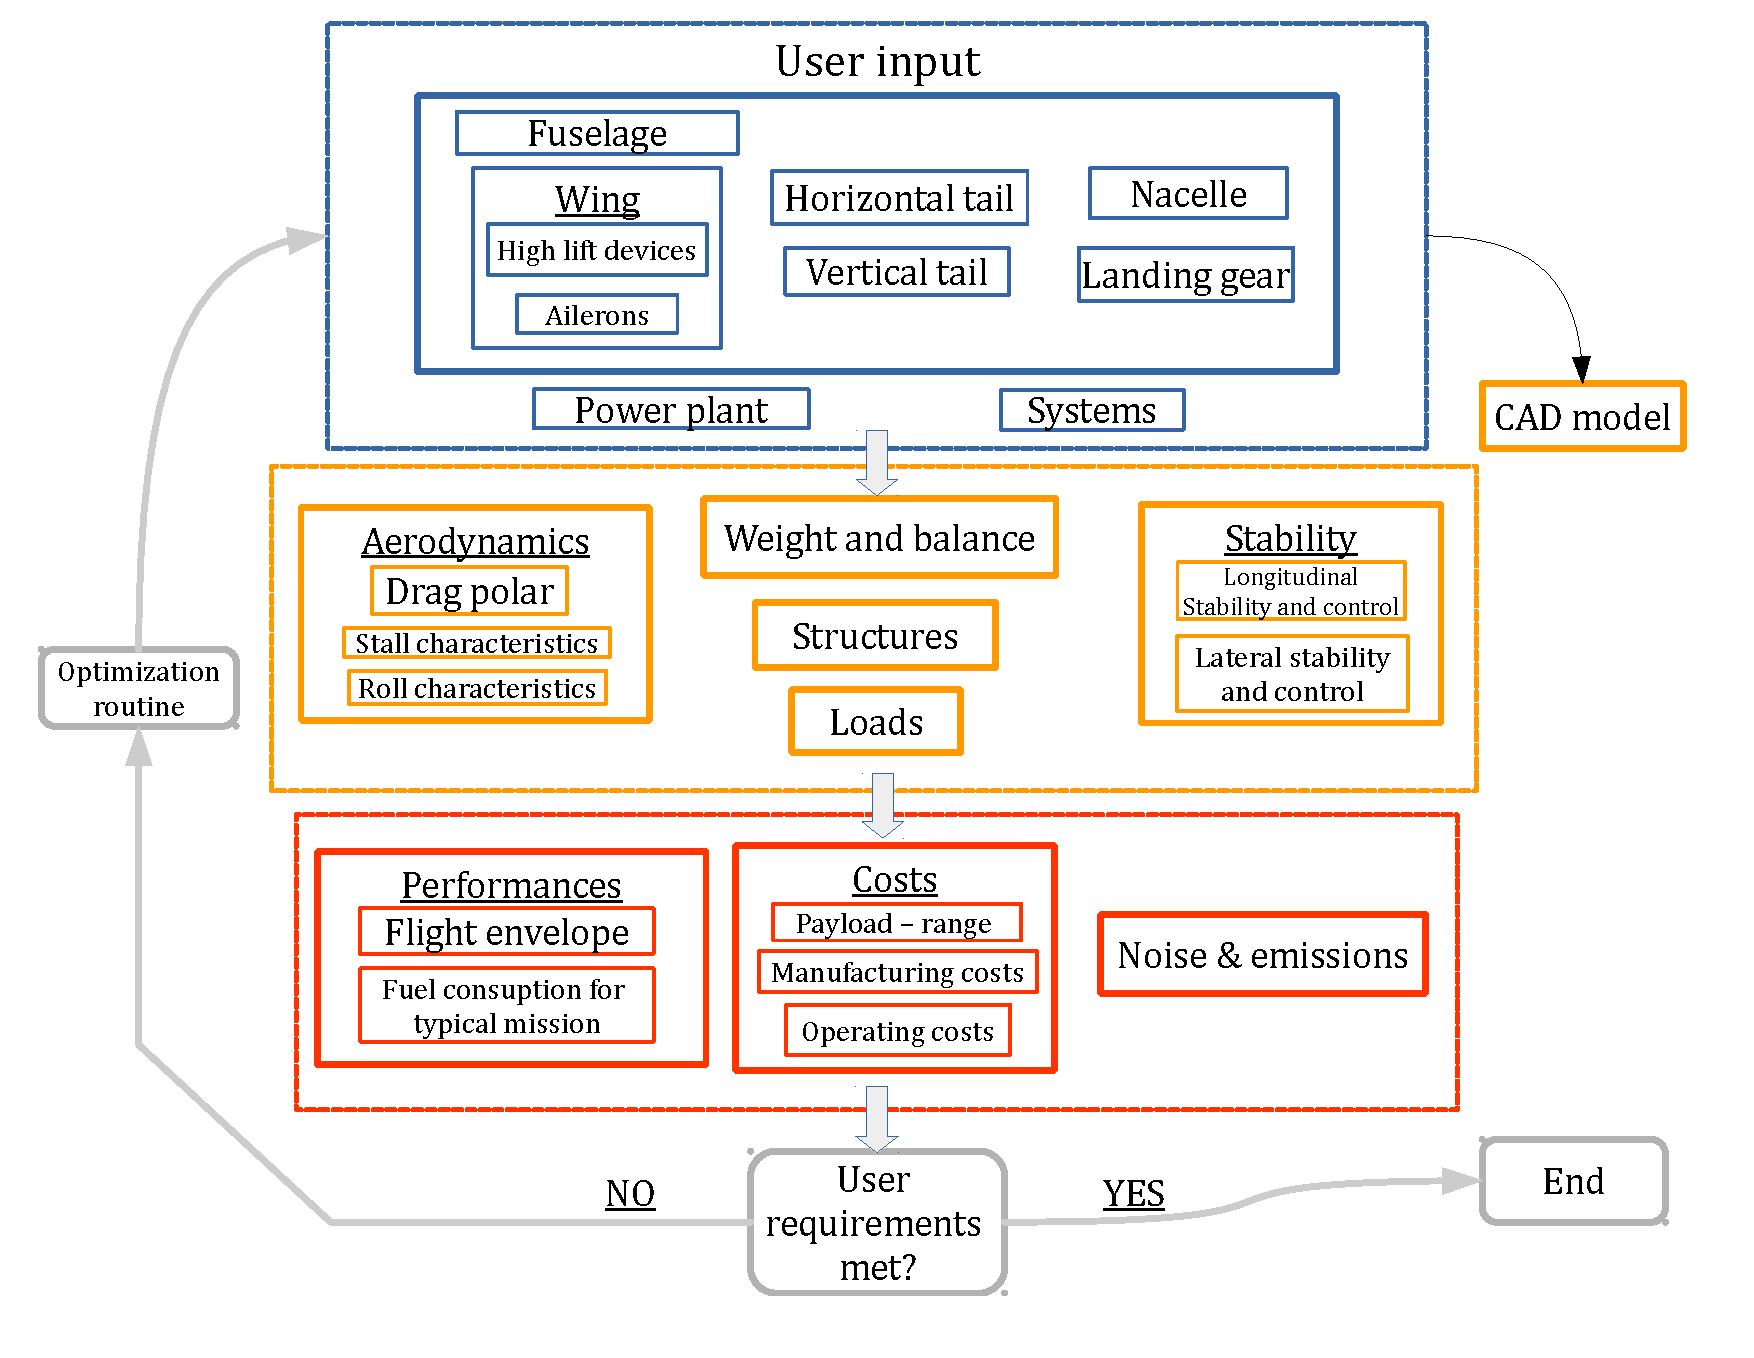
\includegraphics[height = 8.6cm ]{Immagini/flowchart3}
	\caption{Software calculation modules.}
	\label{fig:guiStart}
\end{figure}

\section{Software architecture}

\gls{acr:Jpad} library isactually divided into three package: JPADConfigs, JPADCore and JPADSandbox.  Each package is organized in several classes or more package in order to have a clear and simple classification. The possibility to place similar classes in the same package has been extensively exploited for the same reasons, see section A.2.   The source code has been extensively commented following Javadoc practices. This enabled us to automatically generate documentation using Doxygen \cite{doxgen}

\begin{figure}[H]
	\centering
	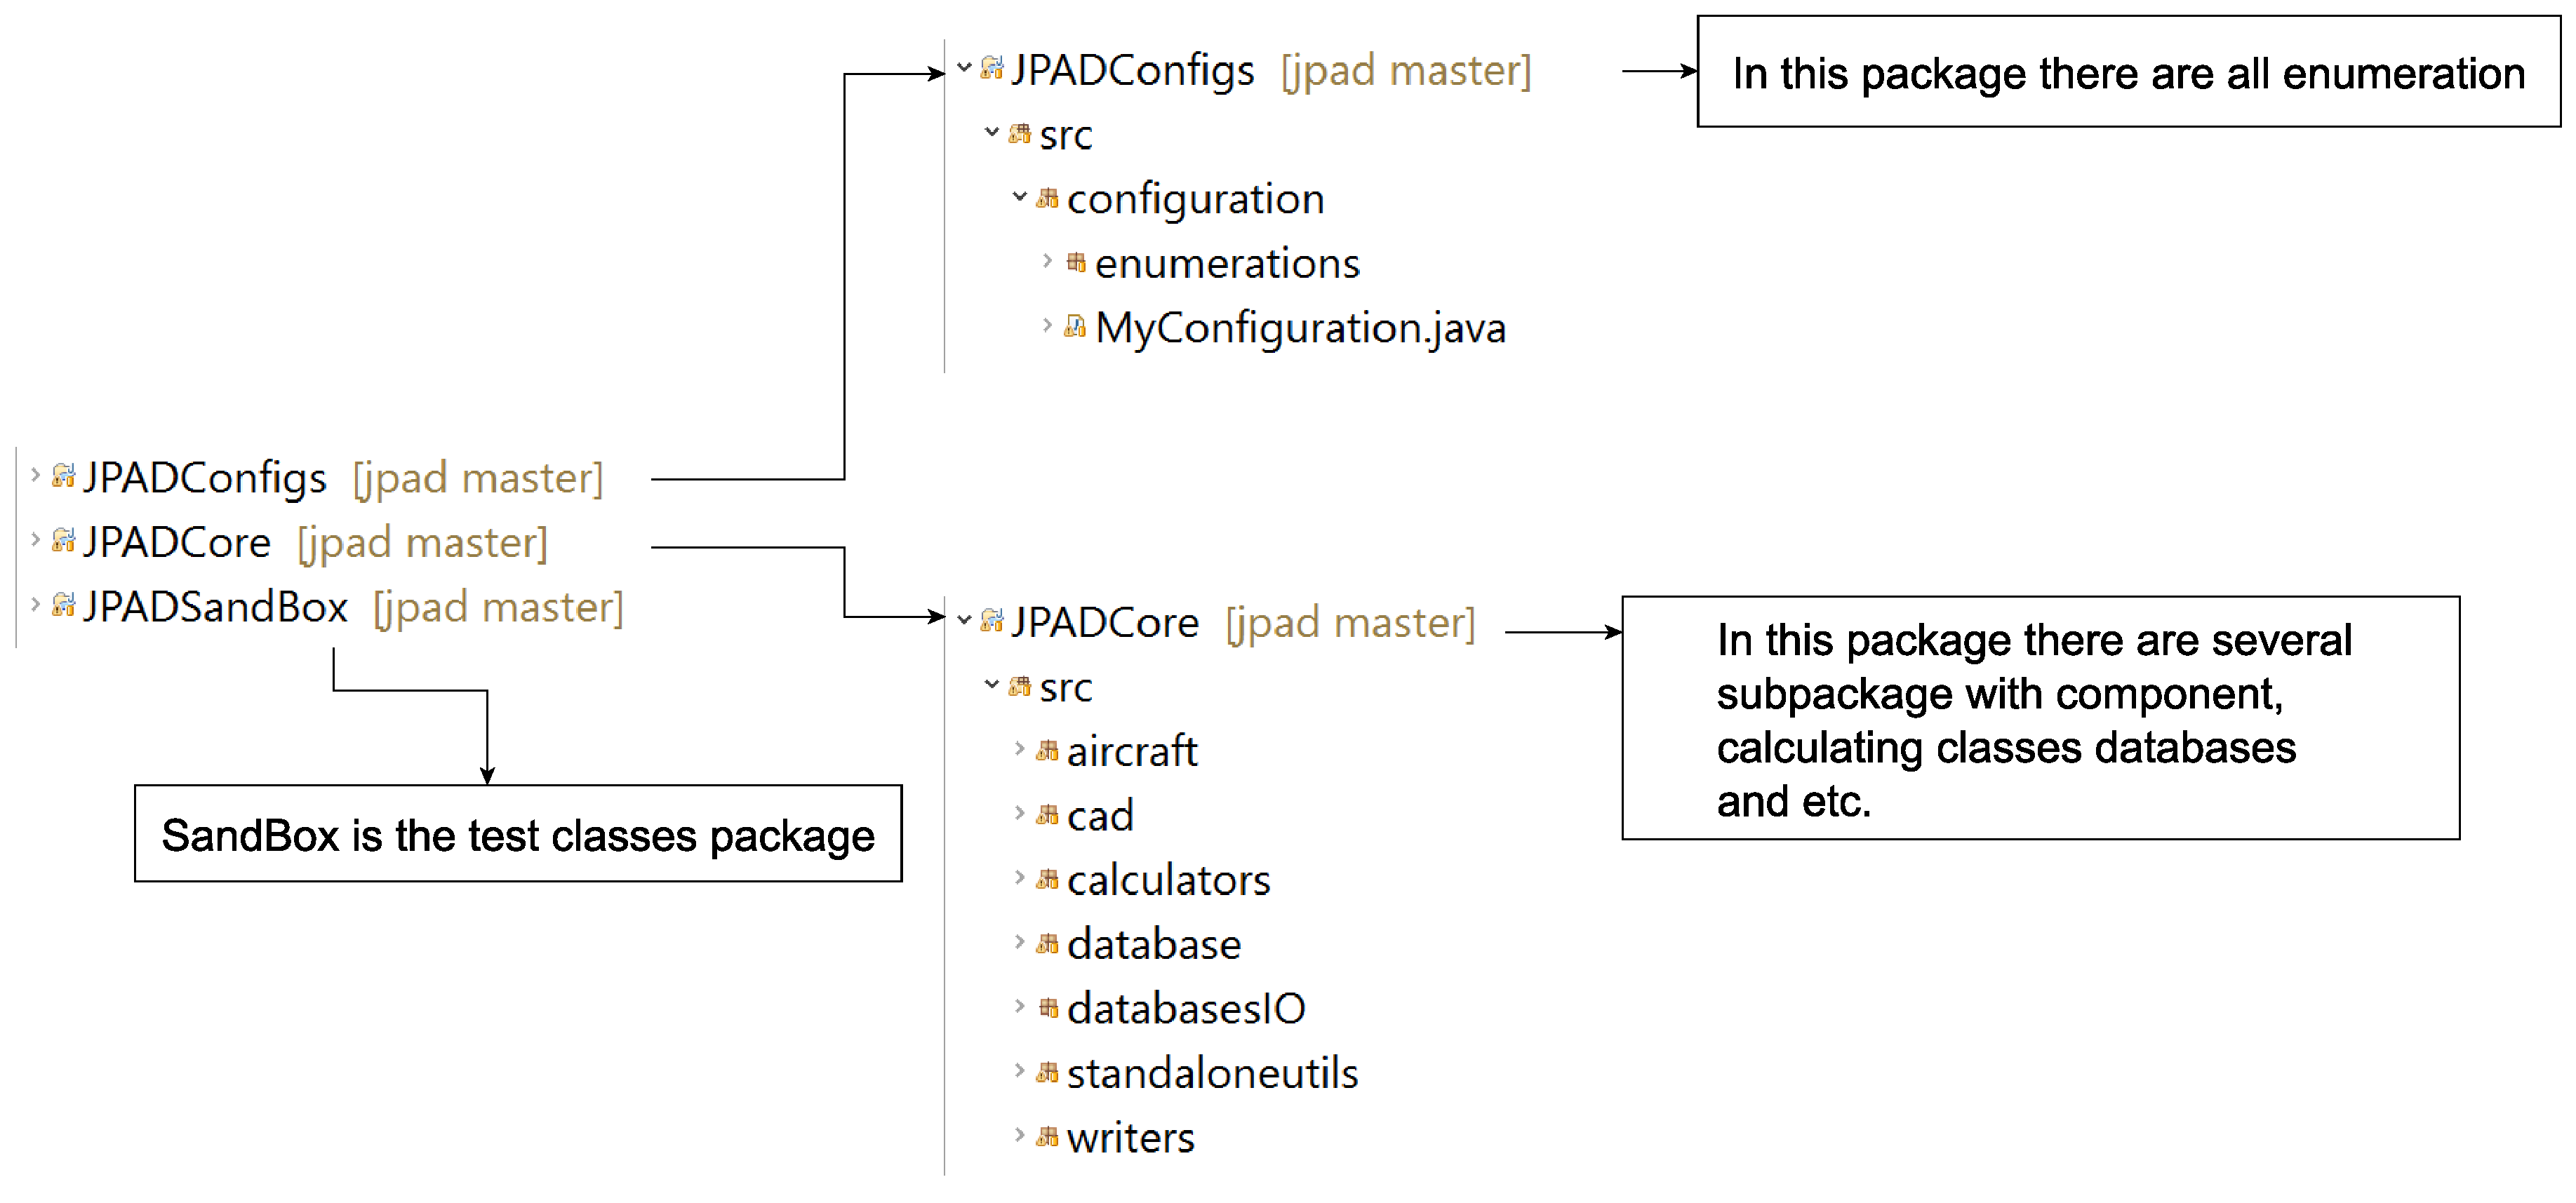
\includegraphics[height = 7.6cm ]{Immagini/organization}
	\caption{Software package division.}
	\label{fig:sw}
\end{figure}
 
 The main package of \gls{acr:Jpad} library is JPADCore where there are all aircraft component, the managers of calculator and  its computers classes. In the following subsection will explained the main packages of JPADCore.
 
 \subsection{Aircraft package}
 Each component (e.g., the fuselage, the wing, the engine) is therefore defined in its own class. In the aircraft package there are other sub-package for components. In each of these there are a class for the object definition and a manager for the analysis. These manager classes uses the utilities located in the calculator package. \\
 The sub-package in the \texttt{aircraft} package are the following:
 
 \begin{itemize}
 \item \texttt{Auxiliary} that manages the airfoils
 \item  \texttt{Component} that contains the \texttt{aircraft} class, the aircraft components packages (fuselage, lifting surfaces, nacelles, power plant, fuel tank, landing gear, systems) and, inside them, their manager analysis classes used to call related analysis methods. 
 \item \texttt{OperatingConditions} 
 \end{itemize}
 
 \noindent \\ \\ 

Basic data for describing the {\bfseries fuselage} are contained in the \texttt{fuselage} class. This holds all the fuselage overall properties, such as the length, maximum width and maximum height, length ratios between the nose and the tail parts length to the constant section part length, number of decks and so on. Other classes in the package manage the shape of fuselage sections and outlines (which define the fuselage shape in the xz and xy planes) and aerodynamics calculations (Aerodynamics class).\\ \\

The data relating to the {\bfseries lifting surfaces} are contained in the \texttt{liftingSurface } class. Since the lifting surfaces of an aircraft share several characteristics, a single class has beencreated to manage the wing, the horizontal and vertical tail and, eventually, the canard. The lifting surface specific category (that is, wing, horizontal tail etc.) is acknowledged through a \texttt{MyComponentEnum} variable which has to be specified when creating the lifting surface object. By default, a lifting surface has three primary span stations: root ($\eta = 0$), middle and tip ($\eta = 1$). The middle station location is user-defined and is used to represent a change in chord.y/ law; such a change can be due to a lifting surface kink or to the beginning of a tapered part. If the wing is simple tapered the middle station can also be omitted.\\ \\

The data relating to the {\bfseries airfoils} are handled by \texttt{Airfoil} class, that creates for each lifting surface three airfoils, located respectively at $\eta=0$, $\eta=1$ and at middle station. An airfoil object holds:
\begin{enumerate}
	\item the position along the semispan, $\eta$;
	\item twist value relative to root, $\epsilon_g$;
	\item zero lift angle of attack, $\alphazlp$;
	\item angle of attack value at the end of the linear part of $C_l(\alpha)$ curve, $\alphastar$;
	\item stall angle of attack, $\alpha_{stall}$;
	\item lift gradient of the linear part of $C_l(\alpha)$ curve, $\Clalphap$;
	\item minimum drag coefficient, $C_{d,min}$;
	\item lift coefficient at $C_{d,min}$, $C_l@C_{d,min}$;
	\item lift cofficient at the end of linear part;
	\item maximum lift coefficient, $\Clmaxp$
	\item drag polar $K$ factor;
	\item aerodynamic moment coefficient gradient, $C_{m_\alpha}$;
	\item aerodynamic center x coordinate, $x_{ac}$;
	\item aerodynamic moment coefficient with respect to the aerodynamic center, $C_{m_{ac}}$ or $\Cmzerop$;
	\item aerodynamic moment coefficient with respect to the aerodynamic center at stall, $C_{m_{ac},stall}$;
	\item maximum thickness to chord ratio, $t/c_{max}$;
	\item x,z non dimensional coordinates.
\end{enumerate}
At the time of writing all these quantities have to be entered by the user. The \texttt{Airfoil} class provides the \texttt{populateCoordinateList()} method which transforms the non dimensional coordinates provided by the user in order to obtain their actual coordinates, which takes into account of actual chord length, ACRF position, sweep, twist and dihedral.\\ \\

The power plant is defined in the package \texttt{PowerPlant} in \texttt{components}. In this package there is the \texttt{engine} class that initializes the data related to the single engine. An other class in the same package, \texttt{powerPlant} creates the parametric model of the power plant using a list of objects creates by \texttt{engine}.



\subsection{\texttt{MyOperatingConditions} class}
As the name suggests, this class contains all the data related to atmosphere conditions (which are currently derived from altitude value using the 1976 ISA model), current speed (Mach number), gravitational acceleration (\SI{9.80665 }{\meter/\second^2}) and sea level pressure (\SI{101325}{\Pa}).

A \texttt{MyOperatingConditions} object can be created regardless of the aircraft configuration as the class is entirely self contained: the aircraft could also be undefined at the time of the object creation. If the user wants to run several analysis at different operating conditions, a \texttt{MyOperatingConditions} instance has to be created for each one.


 \subsection{Calculators package}
 % continua da qua 
 This package includes all the calculators classes. Calculator classes have been created to evaluate quantities related with more than one component. The calculator classes are the following:
 
 \begin{itemize}
 \item {\texttt{AerodynamicCalc} class}: It contains all the necessary methods to evaluate the current configuration aerodynamics, such as the overall $C_{D_0}$ coefficient and the drag polar.
\item {\texttt{MyBalance} class}: It holds the methods for evaluating the current configuration center of gravity and the loading cycle curve.
\item {\texttt{MyPerformances} class}: It holds all performance related calculations such as maximum range, flight envelope and so on.
\item {\texttt{MyWeights} class}: It calls the methods of each component necessary to evaluate the component weight. Since each component's weight can be estimated with several different methods, this class also manages which method have to be used. 
\end{itemize} 


\subsection{Database package}


 \subsection{Writers package}
 



\section{Graphical User Interface (GUI)}
An extensive work has been done to set up an effective Graphical User interface (GUI) to reduce the time the user has to spend to obtain relevant results. The result presented in this section is the early step of graphical interface, which is currently in development.\\ \\

The Java programming language greatly helped to build the GUI: several open source libraries (SWT, JFace) allowed us to build a functional yet pleasant GUI which allows the user to easily change the aircraft’s parameters, to view a 3D model of the defined geometry, to launch a new analysis and view the corresponding results. The current GUI appearance is shown in fig. \ref{fig:guiStart}. It is composed of several items:
\begin{enumerate}
	\item a menu bar (on top), which holds all the available actions divided in sub-categories;
	\item a toolbar (below the menu bar), which holds the most important actions needed to interact with the application. The toolbar, as the menu bar, is always visible to the user;
	\item a project tree (on the left), a key component of the GUI since it provides access to all the components of the aircraft and the analysis results any time during the execution of the application. The project tree appears once an aircraft is created and can be eventually hidden;
	\item a 3D view, which shows the CAD model of the aircraft selected by the user. The CAD model can be updated each time the user wants to check the changes made to the aircraft geometry;
	\item a log message window, placed at the bottom, that tells the user the status of pending operations. This window can be hidden;
	\item a tab folder, which contains all the windows opened using the project tree; these windows can be closed and reopened any time.
\end{enumerate}


\begin{figure}[H]
	\centering
	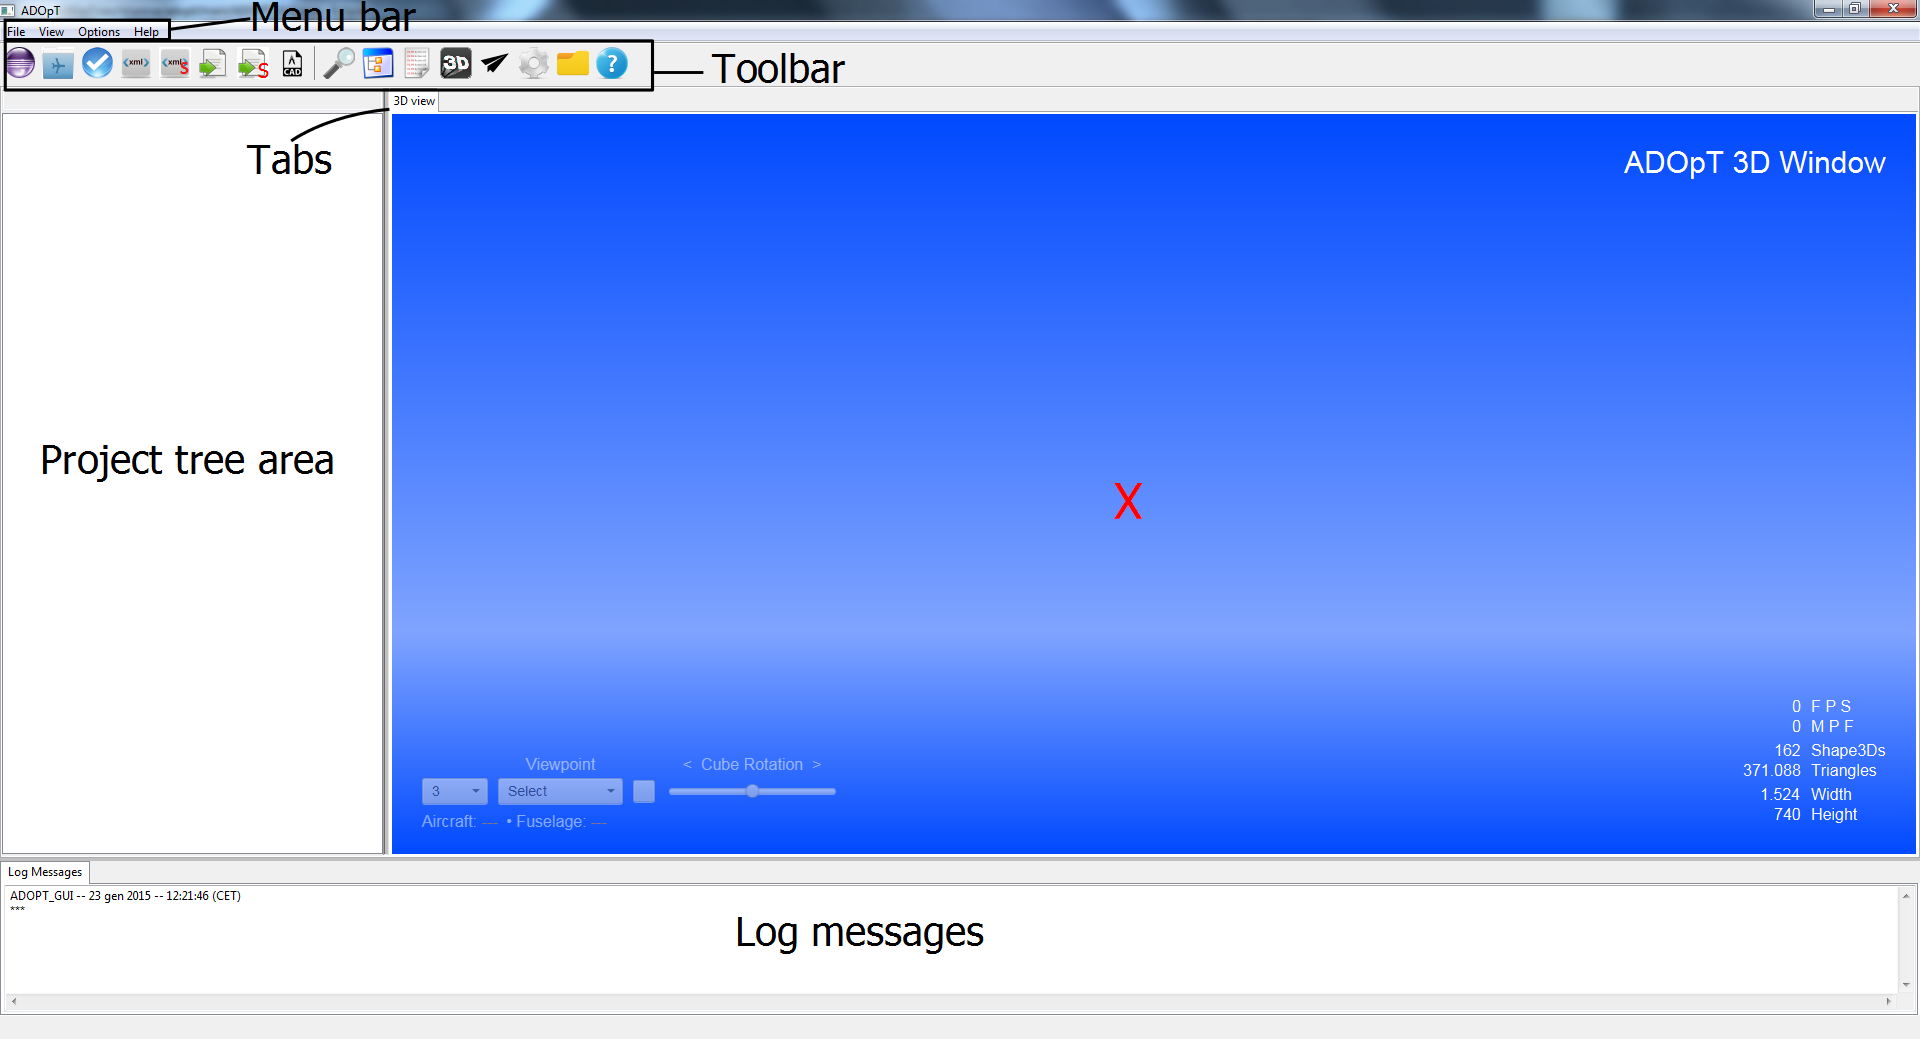
\includegraphics[height = 8cm ]{Immagini/gui/applicationStart.png}
	\caption{The GUI when the application is started.}
	\label{fig:guiStart}
\end{figure}

\subsection{Typical work session}
In developing the application we focused on making the user's typical work session as simple as possible. Few basics steps are required for running an analysis:

\begin{enumerate}
	\item create a new aircraft, which we will call A. This can be done using the corresponding button \big(
\includegraphics[scale=0.6]{Immagini/gui/icons/FolderAirplane_32x32.png}\big) in the toolbar, which instantiates the default aircraft
	
	\item set the parameters that define the aircraft model using the corresponding window opened using the tree

	
	\item explore the 3D model \big(
\includegraphics[scale=1.2]{Immagini/gui/icons/3DView_32x32.png}\big) of the aircraft and eventually change some parameters if there is some error

	
	\item execute a complete analysis \big(
\includegraphics[scale=0.5]{Immagini/gui/icons/analysis_32x32.png}\big) of the aircraft previously defined;

	\item export the analysis results to an XML and/or an XLS file \big(
\includegraphics[scale=0.4]{Immagini/gui/icons/Export_32x32.png}\big);
	
	\item eventually export the CAD model of the aircraft \big(
\includegraphics[scale=1.2]{Immagini/gui/icons/cad_32x32.png}\big);
	\item save the current aircraft to an XML file \big(
\includegraphics[scale=0.4]{Immagini/gui/icons/XML_32x32.png}\big).
\end{enumerate}
%

\begin{figure}[H]
		\centering
		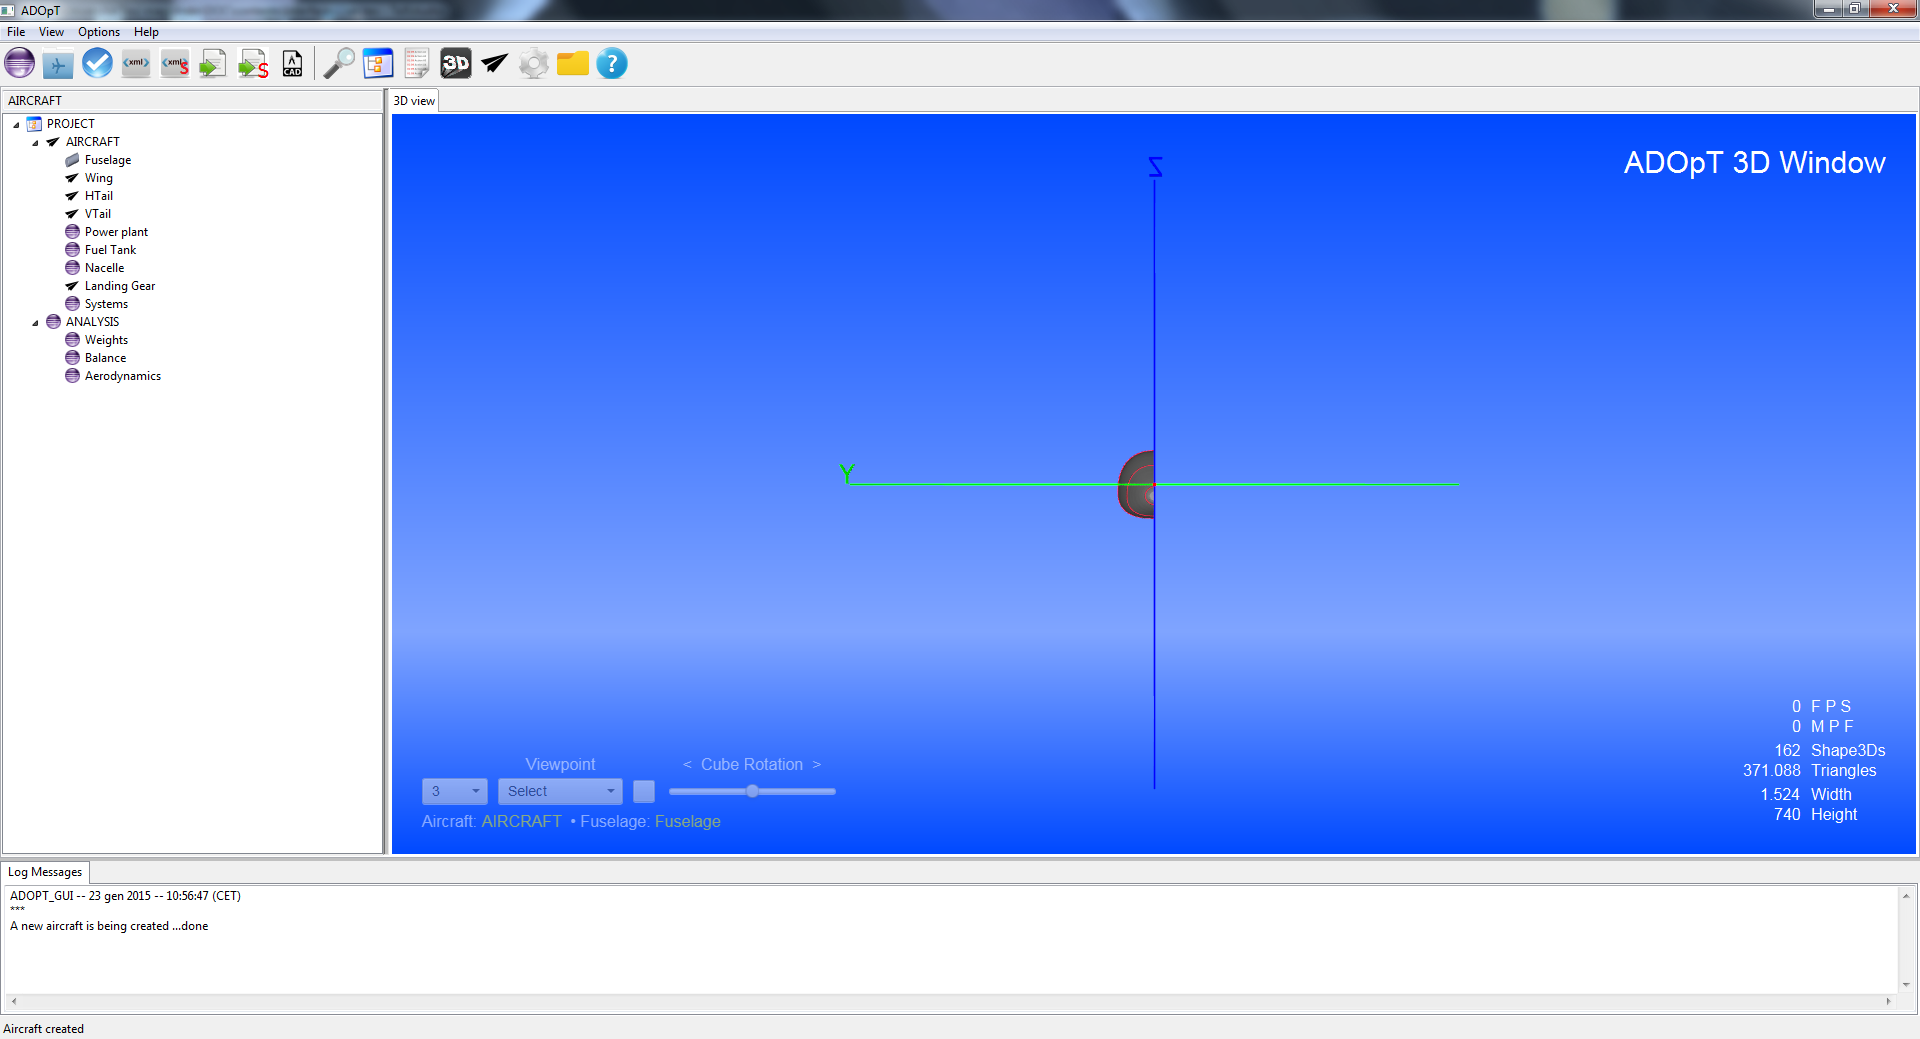
\includegraphics[height = 8cm ]{Immagini/gui/createAircraftDone.png}
		\caption{The GUI as it appears when an aircraft is created.}
		\label{fig:guiDescription}
	\end{figure}
	
	\begin{figure}[H]
		\centering
		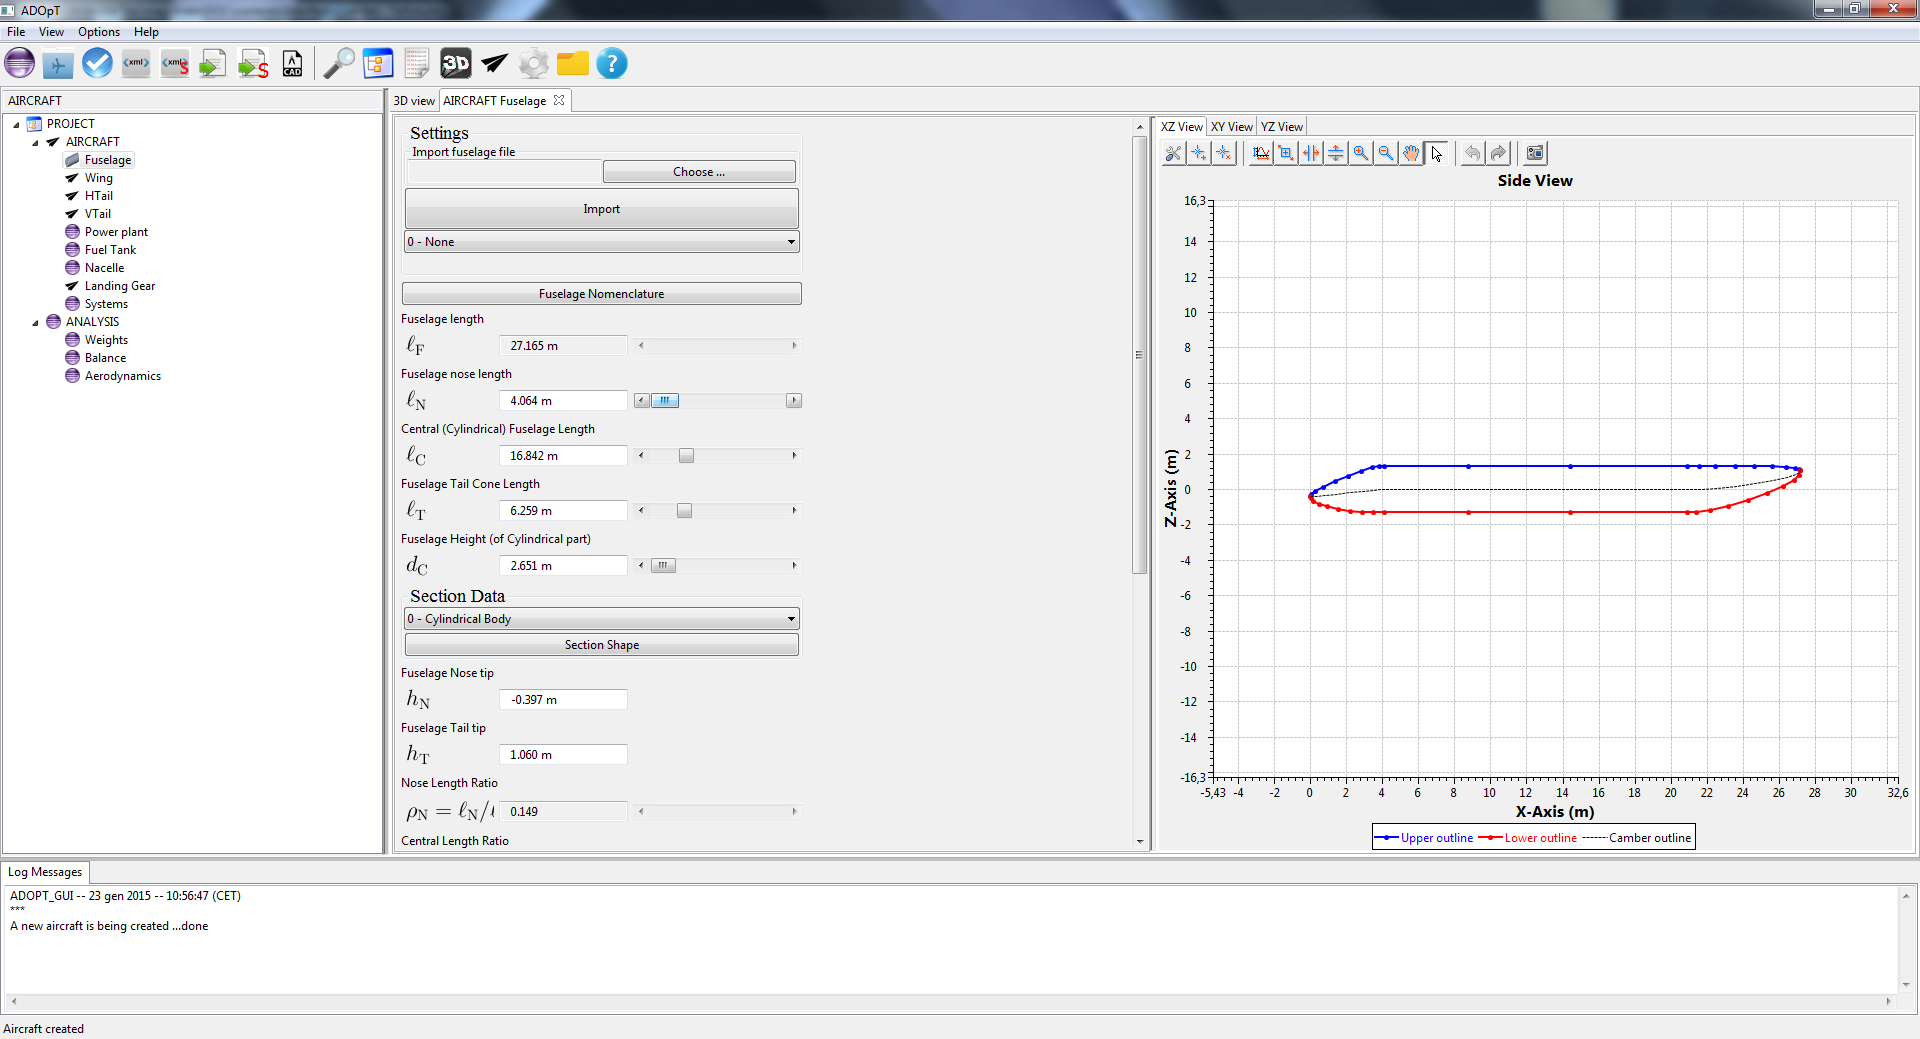
\includegraphics[height = 8cm]{Immagini/gui/changeFusParam.png}
		\caption{The window for changing the fuselage parameters.}
	\end{figure}
	
	\begin{figure}[H]
	\centering
		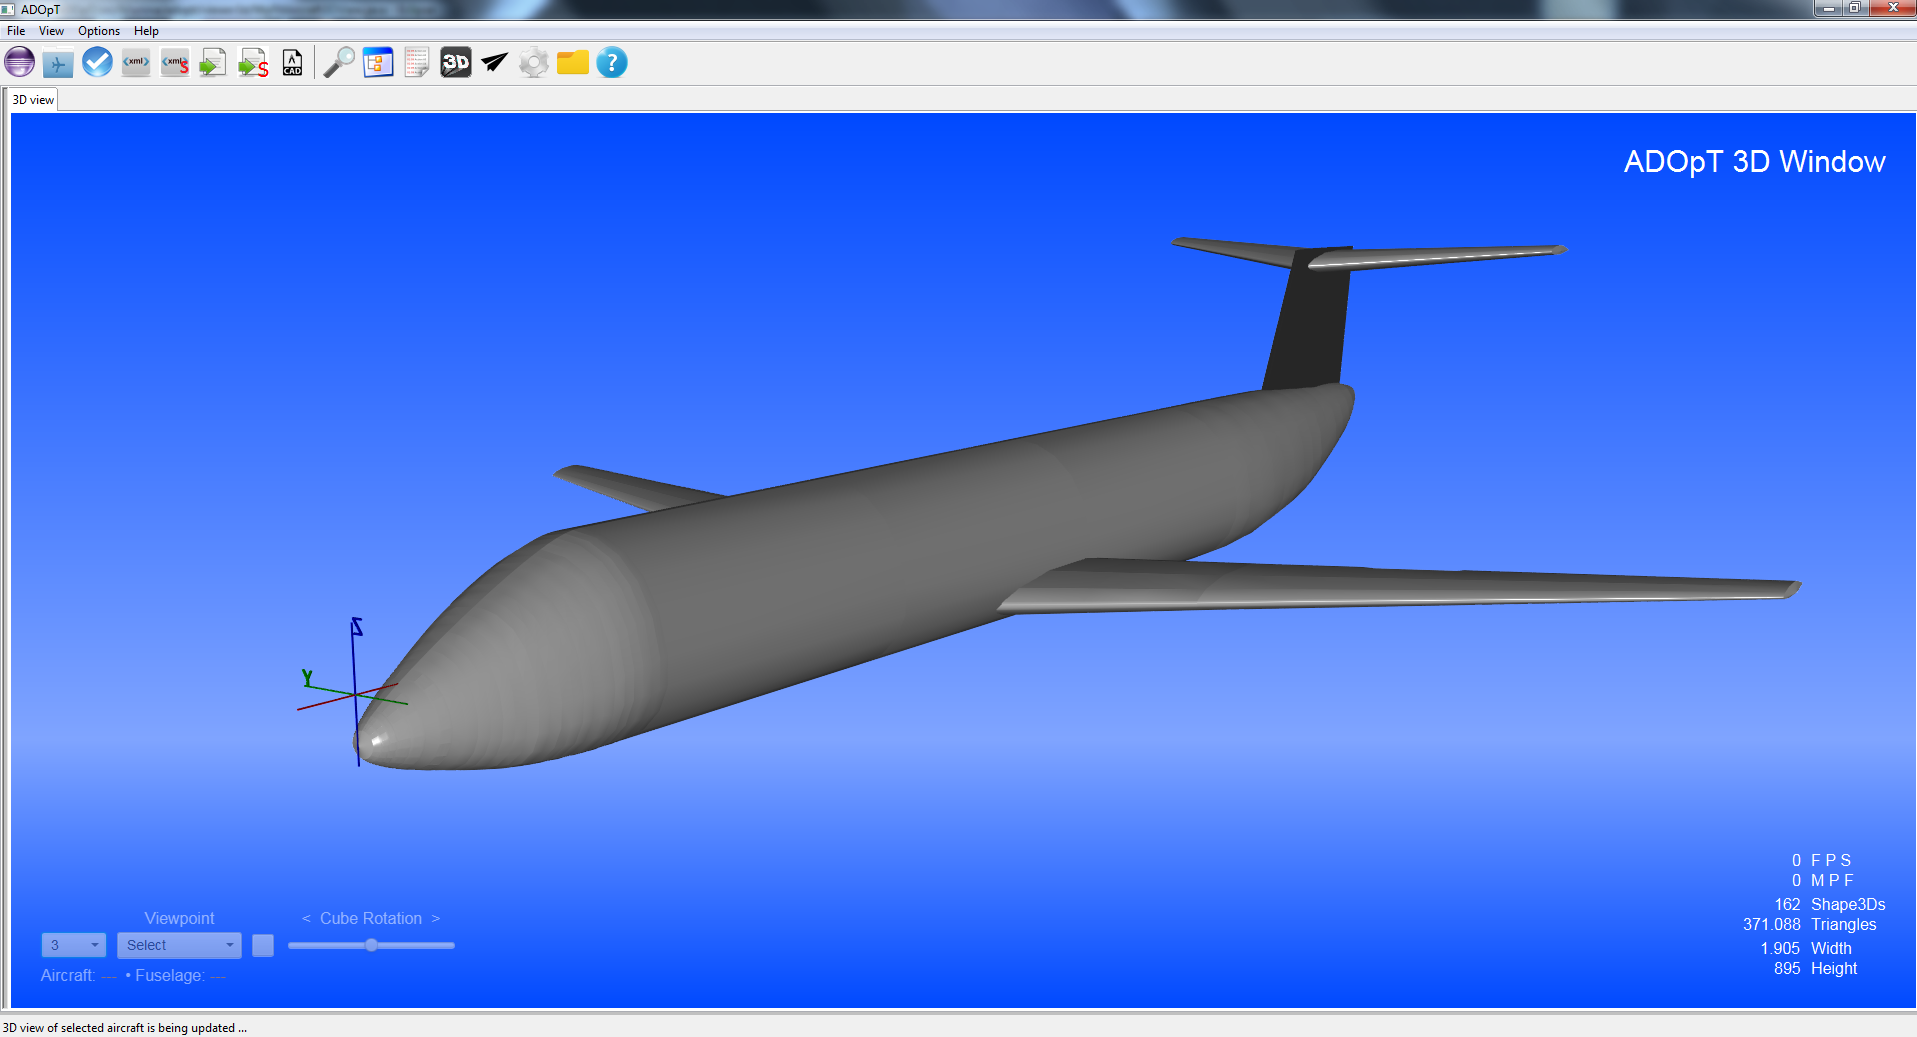
\includegraphics[height =8cm]{Immagini/gui/cad1.png}
		\caption{The aircraft 3D view (log window and project tree hidden).}
	\end{figure}
	
	\begin{figure}[H]
	\centering
		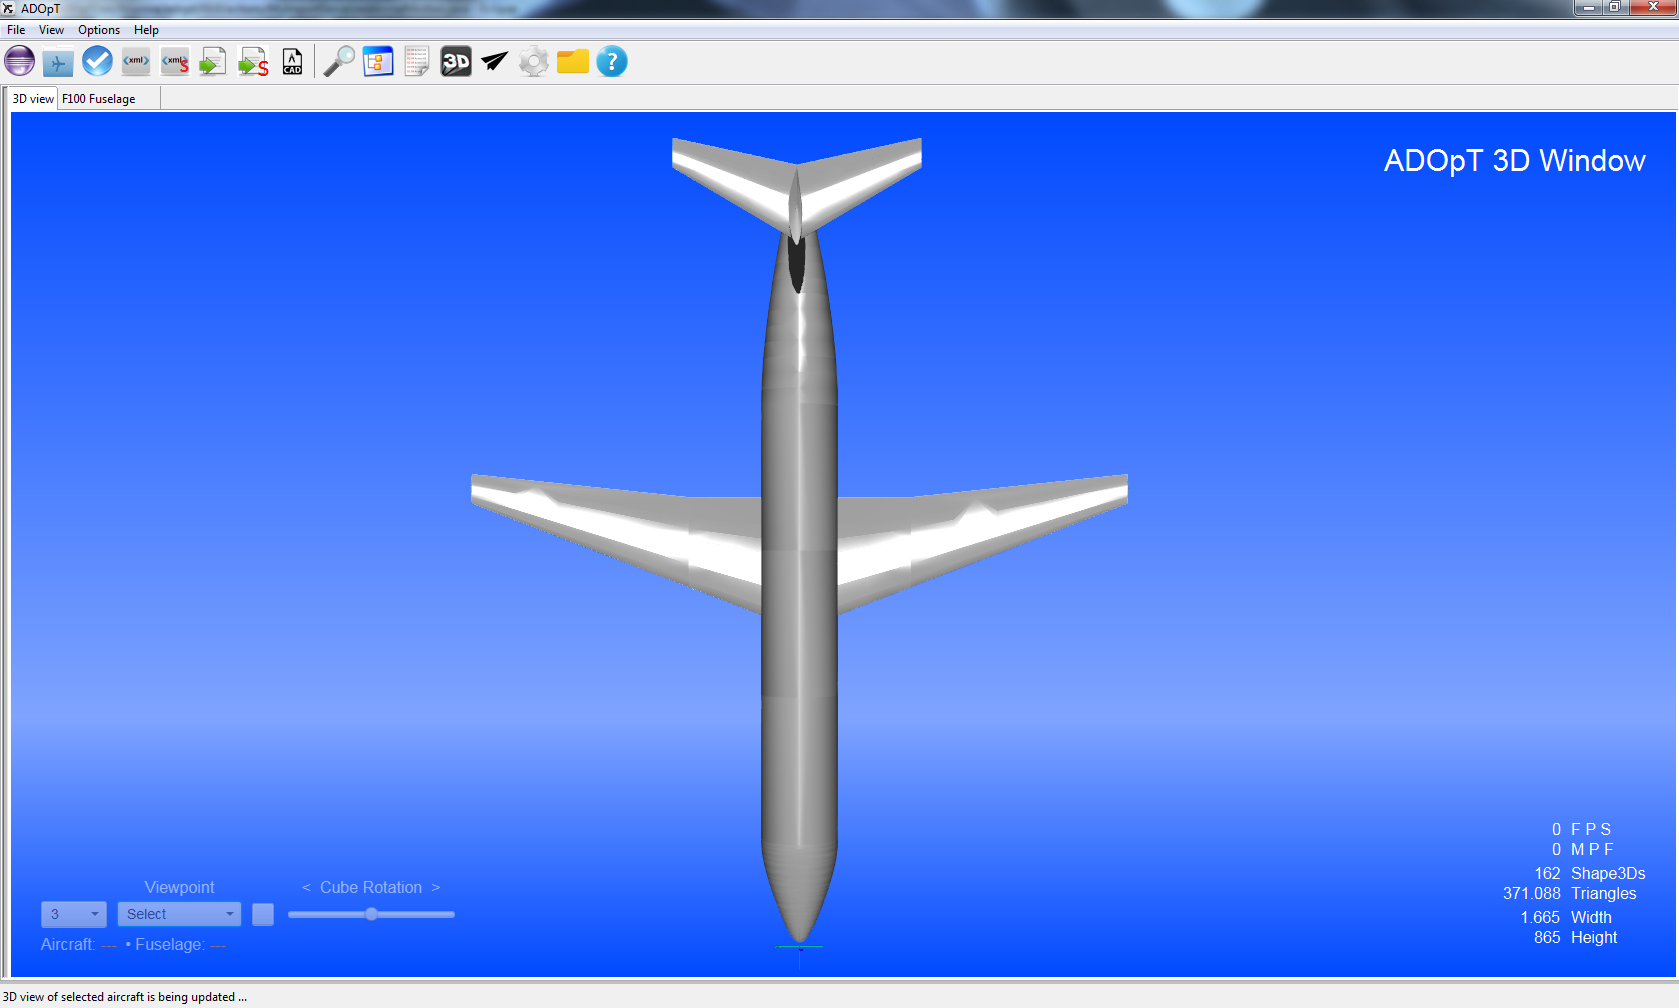
\includegraphics[height =9cm]{Immagini/gui/cad3.png}
		\caption{The aircraft 3D view.}
	\end{figure}

At this point the user could simply change the current configuration until the analysis results are satisfactory. The application can however help the user in finding such a configuration, since it can hold multiple configurations simultaneously, analyse all of them and compare them side by side. To accomplish this task, once the first aircraft has been created, the user should:

\begin{enumerate}
	\item import the aicraft previously saved or create an entirely new aircraft, which we will call B;
	\item change B parameters and run a new analysis on it;
	\item study the results and eventually change some of the parameters;
	\item save every configuration and the corresponding results to file;
	\item export both aircraft and the corresponding results to an XLS file.
\end{enumerate}

\begin{figure}[h]
	\centering
	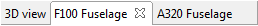
\includegraphics[width=5cm]{Immagini/gui/tabId.png}
	\caption{Same component tab belonging to different aircraft}
	\label{fig:tabId}
\end{figure}

There is no limit to the number of aircraft the application can handle; each aircraft is added to the project tree as shown in fig. \ref{fig:projectTreeMulti} providing access to the corresponding components and analysis.

\begin{figure}[H]
	\centering
	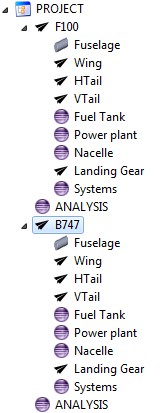
\includegraphics[height=8cm]{Immagini/gui/projectTreeMulti.png}
	\caption{The project tree holding two different aircraft}
	\label{fig:projectTreeMulti}
\end{figure}

\subsection{CAD modelling}
The application can also be used as a basic parametric \gls{acr:cad} modeler. The capability to change the aircraft parameters using the corresponding controls in the \gls{acr:gui}, coupled with the 3D view, allows the user to change each component shape and dimension, view the updated \gls{acr:cad}model and eventually export it to file once some satisfactory results have been obtained.\\

Throughout the development of the application, great care has been given to the making of
the CAD model for several reasons:


\begin{itemize}
\item it enables the user and the user developer to have an immediate feedback about the data provided to the application: if some geometrical parameter is wrong, the CAD model makes it impossible not noticing it;
\item  it allows the user to run a CFD analysis with an external program. The CAD model has been in fact built so that it is ready to be meshed by an external mesher without any kind of adjustment;
\item it provides an accurate estimate of the wetted surface of each component.
\end{itemize}

The creation of the CAD model was made possible by the occjava library, whose classes and methods have been used to build each component’s model. The CAD model can be saved in two different file formats: STEP and BREP; they have proven to take both little memory and to give the best results in terms of geometry representation. The IGES format gave instead mixed results so we preferred to use only the first two.

\begin{figure}[H]
	\centering
		\includegraphics[width=6 cm]{Immagini/gui/CADfuselageTailBAD2.png}
		\caption{A detail of the tail of the fuselage obtained as a unique loft}
		\label{fig:badTail}
	\end{figure}
	
	\begin{figure}[H]
	\centering
		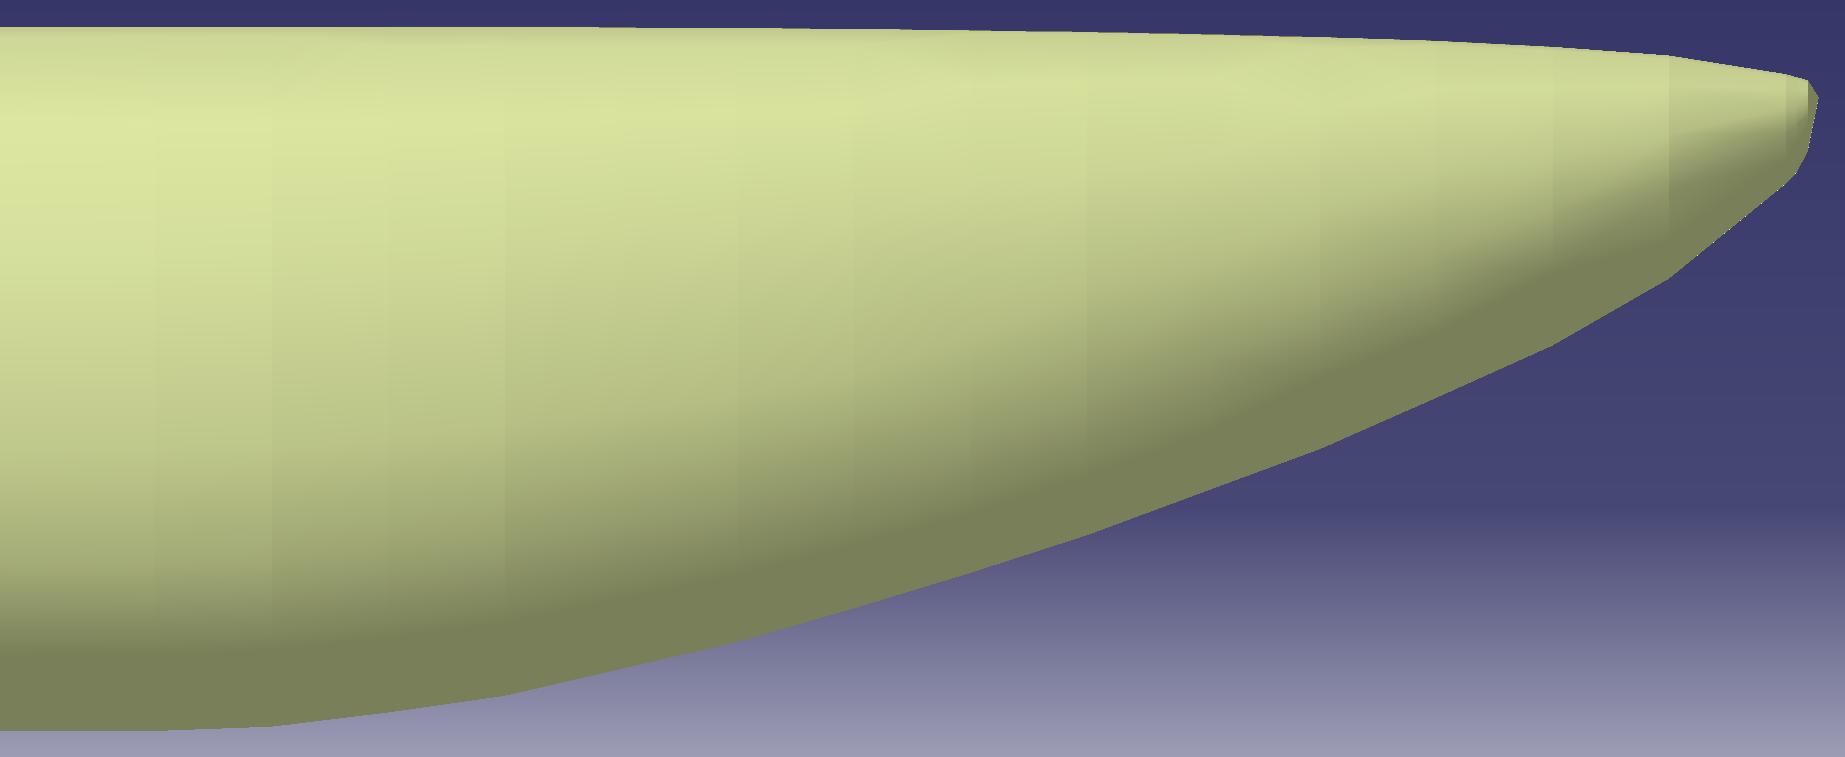
\includegraphics[width=6 cm]{Immagini/gui/CADfuselageTailOK.png}
		\caption{A detail of the tail of the fuselage obtained sewing together its parts}
		\label{fig:goodTail}
\end{figure}


\section{In Development}